\section{Connections and curvature}

\subsection{The function \texorpdfstring{\( T \)}{T}}

We will build up a map \( T \) out of \( \oo \) which is meant to be like the circle bundle of a tangent bundle. And so we will begin with the intrinsic data of the link at each point: taking the link of a vertex gives us a map from vertices to polygons.

\begin{mydef}
\( T_0\defeq\link:\oo_0\to\EMzo \) is given by:
\begin{align*}
\link(w) &= brgo & \link(r) &= wbyg \\
\link(y) &= bogr & \link(g) &= wryo \\
\link(b) &= woyr & \link(o) &= wgyb
\end{align*}
We chose these orderings for the vertices in the link, by visualizing standing at the given vertex as if it were the north pole, then looking south and enumerating the link in clockwise order, starting from \( w \) if possible, else \( b \).
\end{mydef}

\begin{figure}[htbp]
\centering
\begin{figure}[h]
\centering
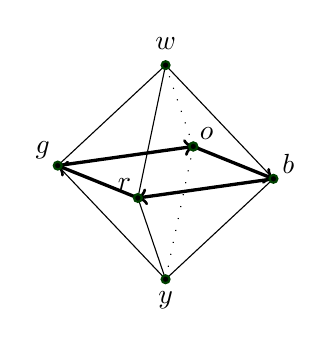
\begin{tikzpicture}%
  [x={(-0.860769cm, -0.121512cm)},
  y={(0.508996cm, -0.205391cm)},
  z={(-0.000053cm, 0.971107cm)},
  scale=1,
  eqback/.style={->, very thick},
  back/.style={loosely dotted, thin},
  eqedge/.style={->, very thick},
  edge/.style={black, thin},
  facet/.style={fill=blue!95!black,fill opacity=0.0},
  vertex/.style={inner sep=1pt,circle,draw=green!25!black,fill=black,thick}]
\coordinate (-1, -1, 0) at (-1, -1, 0);
\coordinate (-1, 1, 0) at (-1, 1, 0);
\coordinate (0, 0, -1) at (0, 0, -1);
\coordinate (0, 0, 1) at (0, 0, 1);
\coordinate (1, -1, 0) at (1, -1, 0);
\coordinate (1, 1, 0) at (1, 1, 0);
%% Drawing edges in the back
%%
\draw[edge,eqback] (-1, -1, 0) -- (-1, 1, 0);
\draw[edge,back] (-1, -1, 0) -- (0, 0, -1.4);
\draw[edge,back] (-1, -1, 0) -- (0, 0, 1.4);
\draw[edge,eqback] (1, -1, 0) -- (-1, -1, 0);
%% Drawing vertices in the back
%%
\node[vertex] at (-1, -1, 0)     {};
%% Drawing the facets
%%
\fill[facet] (1, 1, 0) -- (0, 0, -1.4) -- (1, -1, 0) -- cycle {};
\fill[facet] (1, 1, 0) -- (0, 0, 1.4) -- (1, -1, 0) -- cycle {};
\fill[facet] (1, 1, 0) -- (-1, 1, 0) -- (0, 0, 1.4) -- cycle {};
\fill[facet] (1, 1, 0) -- (-1, 1, 0) -- (0, 0, -1.4) -- cycle {};
%% Drawing edges in the front
%%
\draw[edge] (-1, 1, 0) -- (0, 0, -1.4);
\draw[edge] (-1, 1, 0) -- (0, 0, 1.4);
\draw[eqedge] (-1, 1, 0) -- (1, 1, 0);
\draw[edge] (0, 0, -1.4) -- (1, -1, 0);
\draw[edge] (0, 0, -1.4) -- (1, 1, 0);
\draw[edge] (0, 0, 1.4) -- (1, -1, 0);
\draw[edge] (0, 0, 1.4) -- (1, 1, 0);
\draw[eqedge] (1, 1, 0) -- (1, -1, 0);
%% Drawing the vertices in the front
%%
\begin{scope}[nodes=vertex]
\node[label=above right:\( b \)] at (-1, 1, 0)     {};
\node[label=below:\( y \)] at (0, 0, -1.4)     {};
\node[label=above:\( w \)] at (0, 0, 1.4)     {};
\node[label=above left:\( g \)] at (1, -1, 0)     {};
\node[label=above left:\( r \)] at (1, 1, 0)     {};
\node[label=above right:\( o \)] at (-1, -1, 0)     {};
\end{scope}
\end{tikzpicture}

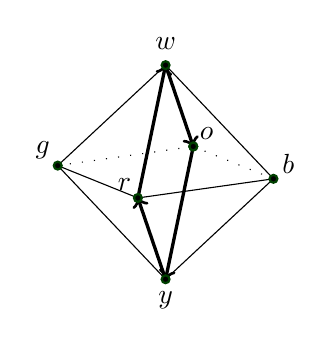
\begin{tikzpicture}%
  [x={(-0.860769cm, -0.121512cm)},
  y={(0.508996cm, -0.205391cm)},
  z={(-0.000053cm, 0.971107cm)},
  scale=1,
  eqback/.style={->, very thick},
  back/.style={loosely dotted, thin},
  eqedge/.style={->, very thick},
  edge/.style={black, thin},
  facet/.style={fill=blue!95!black,fill opacity=0.0},
  vertex/.style={inner sep=1pt,circle,draw=green!25!black,fill=black,thick}]
\coordinate (-1, -1, 0) at (-1, -1, 0);
\coordinate (-1, 1, 0) at (-1, 1, 0);
\coordinate (0, 0, -1) at (0, 0, -1);
\coordinate (0, 0, 1) at (0, 0, 1);
\coordinate (1, -1, 0) at (1, -1, 0);
\coordinate (1, 1, 0) at (1, 1, 0);
%% Drawing edges in the back
%%
\draw[edge,back] (-1, -1, 0) -- (-1, 1, 0);
\draw[edge,eqback] (-1, -1, 0) -- (0, 0, -1.4);
\draw[edge,eqback] (0, 0, 1.4) -- (-1, -1, 0);
\draw[edge,back] (1, -1, 0) -- (-1, -1, 0);
%% Drawing vertices in the back
%%
\node[vertex] at (-1, -1, 0)     {};
%% Drawing the facets
%%
\fill[facet] (1, 1, 0) -- (0, 0, -1.4) -- (1, -1, 0) -- cycle {};
\fill[facet] (1, 1, 0) -- (0, 0, 1.4) -- (1, -1, 0) -- cycle {};
\fill[facet] (1, 1, 0) -- (-1, 1, 0) -- (0, 0, 1.4) -- cycle {};
\fill[facet] (1, 1, 0) -- (-1, 1, 0) -- (0, 0, -1.4) -- cycle {};
%% Drawing edges in the front
%%
\draw[edge] (-1, 1, 0) -- (0, 0, -1.4);
\draw[edge] (-1, 1, 0) -- (0, 0, 1.4);
\draw[edge] (-1, 1, 0) -- (1, 1, 0);
\draw[edge] (0, 0, -1.4) -- (1, -1, 0);
\draw[eqedge] (0, 0, -1.4) -- (1, 1, 0);
\draw[edge] (0, 0, 1.4) -- (1, -1, 0);
\draw[eqedge] (1, 1, 0) -- (0, 0, 1.4) ;
\draw[edge] (1, 1, 0) -- (1, -1, 0);
%% Drawing the vertices in the front
%%
\begin{scope}[nodes=vertex]
\node[label=above right:\( b \)] at (-1, 1, 0)     {};
\node[label=below:\( y \)] at (0, 0, -1.4)     {};
\node[label=above:\( w \)] at (0, 0, 1.4)     {};
\node[label=above left:\( g \)] at (1, -1, 0)     {};
\node[label=above left:\( r \)] at (1, 1, 0)     {};
\node[label=above right:\( o \)] at (-1, -1, 0)     {};
\end{scope}
\end{tikzpicture}

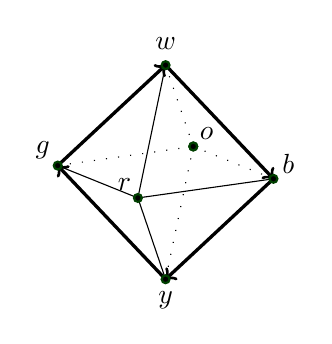
\begin{tikzpicture}%
  [x={(-0.860769cm, -0.121512cm)},
  y={(0.508996cm, -0.205391cm)},
  z={(-0.000053cm, 0.971107cm)},
  scale=1,
  eqback/.style={->, very thick},
  back/.style={loosely dotted, thin},
  eqedge/.style={->, very thick},
  edge/.style={black, thin},
  facet/.style={fill=blue!95!black,fill opacity=0.0},
  vertex/.style={inner sep=1pt,circle,draw=green!25!black,fill=black,thick}]
\coordinate (-1, -1, 0) at (-1, -1, 0);
\coordinate (-1, 1, 0) at (-1, 1, 0);
\coordinate (0, 0, -1) at (0, 0, -1);
\coordinate (0, 0, 1) at (0, 0, 1);
\coordinate (1, -1, 0) at (1, -1, 0);
\coordinate (1, 1, 0) at (1, 1, 0);
%% Drawing edges in the back
%%
\draw[edge,back] (-1, -1, 0) -- (-1, 1, 0);
\draw[edge,back] (-1, -1, 0) -- (0, 0, -1.4);
\draw[edge,back] (-1, -1, 0) -- (0, 0, 1.4);
\draw[edge,back] (1, -1, 0) -- (-1, -1, 0);
%% Drawing vertices in the back
%%
\node[vertex] at (-1, -1, 0)     {};
%% Drawing the facets
%%
\fill[facet] (1, 1, 0) -- (0, 0, -1.4) -- (1, -1, 0) -- cycle {};
\fill[facet] (1, 1, 0) -- (0, 0, 1.4) -- (1, -1, 0) -- cycle {};
\fill[facet] (1, 1, 0) -- (-1, 1, 0) -- (0, 0, 1.4) -- cycle {};
\fill[facet] (1, 1, 0) -- (-1, 1, 0) -- (0, 0, -1.4) -- cycle {};
%% Drawing edges in the front
%%
\draw[eqedge] (-1, 1, 0) -- (0, 0, -1.4);
\draw[eqedge] (0, 0, 1.4) -- (-1, 1, 0);
\draw[edge] (-1, 1, 0) -- (1, 1, 0);
\draw[eqedge] (0, 0, -1.4) -- (1, -1, 0);
\draw[edge] (0, 0, -1.4) -- (1, 1, 0);
\draw[eqedge] (1, -1, 0) -- (0, 0, 1.4);
\draw[edge] (0, 0, 1.4) -- (1, 1, 0);
\draw[edge] (1, 1, 0) -- (1, -1, 0);
%% Drawing the vertices in the front
%%
\begin{scope}[nodes=vertex]
\node[label=above right:\( b \)] at (-1, 1, 0)     {};
\node[label=below:\( y \)] at (0, 0, -1.4)     {};
\node[label=above:\( w \)] at (0, 0, 1.4)     {};
\node[label=above left:\( g \)] at (1, -1, 0)     {};
\node[label=above left:\( r \)] at (1, 1, 0)     {};
\node[label=above right:\( o \)] at (-1, -1, 0)     {};
\end{scope}
\end{tikzpicture}
\caption{The equators for \( w, b, r \).}
\end{figure}
\caption{\( \link \) for the vertices \( w, b\) and \( r \).}
\label{fig:triangle_of_equators}
\end{figure}

To extend \( T_0 \) to a function \( T_1 \) on the 1-skeleton we have complete freedom. Defining a map by induction makes clear that the action on paths is its own structure. Two functions on the octahedron could agree on points but differ on edges. We are going to identify this 1-dimensional freedom with a connection:

\begin{mydef}
\label{def:connection}
A \defemph{connection} on a higher combinatorial manifold is an extension of a circle bundle from the 0-skeleton to the 1-skeleton.
\end{mydef}

Continuing the example, we will do something ``tangent bundley'', imagining how \( T_1 \) changes as we slide from point to point in the embedding shown in the figures. Sliding from \( w \) to \( b \) and tipping the link as we go, we see \( r\mapsto r \) and \( o\mapsto o \) because those lie on the axis of rotation. Then \( g\mapsto w \) and \( b\mapsto y \). 

\begin{mydef}
Define \( T_1:\oo_1\to\EMzo \) on just the 1-skeleton by extending \( T_0 \) as follows:
Transport away from \( w \):
\begin{itemize}
\item \( T_1(wb):[b, r, g, o]\mapsto [y, r, w, o] \) (\( r, o \) fixed)
\item \( T_1(wr):[b, r, g, o]\mapsto [b, y, g, w] \) (\( b, g \) fixed)
\item \( T_1(wg):[b, r, g, o]\mapsto [w, r, y, o] \)
\item \( T_1(wo):[b, r, g, o]\mapsto [b, w, g, y] \)
\end{itemize}
Transport away from \( y \):
\begin{itemize}
\item \( T_1(yb):[b, o, g, r]\mapsto [w, o, y, r] \)
\item \( T_1(yr):[b, o, g, r]\mapsto [b, y, g, w] \)
\item \( T_1(yg):[b, o, g, r]\mapsto [y, o, w, r] \)
\item \( T_1(yo):[b, o, g, r]\mapsto [b, w, g, y] \)
\end{itemize}
Transport along the equator:
\begin{itemize}
\item \( T_1(br):[w, o, y, r]\mapsto [w, b, y, g] \) 
\item \( T_1(rg):[w, b, y, g]\mapsto [w, r, y, o] \)
\item \( T_1(go):[w, r, y, o]\mapsto [w, g, y, b] \)
\item \( T_1(ob):[w, g, y, b]\mapsto [w, o, y, r] \)
\end{itemize}
\end{mydef}

It's very important to be able to visualize what \( T_1 \) does to triangular paths such as \( wb\cdot br\cdot rw \) (which circulates around the boundary of face \( wbr \)). You can see it if you imagine Figure~\ref{fig:triangle_of_equators} as the frames of a short movie. Or you can place your palm over the top of a cube and note where your fingers are pointing, then slide your hand to an equatorial face, then along the equator, then back to the top. The answer is: you come back rotated clockwise by a quarter-turn. 

\begin{mydef}
The map \( R:C_4\to C_4 \) rotates by one quarter turn, one ``click":
\begin{multicols}{2}
\begin{itemize}
\item \( R(c_1) = c_2 \)
\item \( R(c_2) = c_3 \)
\item \( R(c_3) = c_4 \)
\item \( R(c_4) = c_1 \)
\item \( R(c_1c_2) = c_2c_3 \)
\item \( R(c_2c_3) = c_3c_4 \)
\item \( R(c_3c_4) = c_4c_1 \)
\item \( R(c_4c_1) = c_1c_2 \)
\end{itemize}
\end{multicols}
\end{mydef}

Note by univalence the equivalence \( R \) gives a loop in the universe, a term of \( C_4=_{\EMzo}C_4 \).

Now let's extend \( T_1 \) to all of \( \oo \) by providing values for the eight faces. The face \( wbr \) is a path from \( \refl_w \) to the concatenation \( wb\cdot br\cdot rw \), and so the image of \( wbr \) under the extended version of \( T_1 \) must be a homotopy from \( \refl_{T_1(w)} \) to \( T_1(wb\cdot br\cdot rw) \). Here \emph{there is no additional freedom}.

\begin{mydef}
Define \( T_2:\oo\to\EMzo \) by extending \( T_1 \) to the faces as follows:
\begin{multicols}{2}
\begin{itemize}
\item \( T_2(wbr)=H_R \) 
\item \( T_2(wrg)=H_R \)
\item \( T_2(wgo)=H_R \)
\item \( T_2(ybo)=H_R \)
\item \( T_2(yrb)=H_R \) 
\item \( T_2(ygr)=H_R \)
\item \( T_2(yog)=H_R \)
\item \( T_2(ybo)=H_R \)
\end{itemize}
\end{multicols}
where \( H_R:R=\refl_{C_4} \) is the obvious homotopy given by composition with \( R^{-1} \). Passing through univalence we get a 2-path between \( R \) and \( \refl \) in the loop space \( C_4=_{\EMzo}C_4 \).
\end{mydef}

\begin{mydef}
\label{def:curvature}
The \defemph{curvature of a connection} on a family \( T:\mm\to\uni \) at a vertex \( v \) of a 2-face \( f \) with boundary path \( p_f \) of a marked presented type \( \mm \) is the automorphism \( \tr(p_f)(Tv) \) together with a homotopy to \( \id_{Tv} \). Since curvature is a proof that the holonomy is the identity, we may also call it a \defemph{flatness structure}.
\end{mydef}

\begin{mynote}
We have defined a function on a cell by requiring it to correspond to the value on the boundary of that cell. This is familiar in classical differential topology, where it's called \emph{the exterior derivative}. The duality of \( d \) and \( \partial \) is recognizable in \( T_2 \), and we might say ``curvature is the derivative of the connection.''
\end{mynote}

\subsection{Total curvature}
\chcomment[id=Greg]{This subsection is new}
\begin{mydef}
The \defemph{triangular lasso \( L:\Type \) with tail of length \( n \)} (Figure~\ref{fig:lasso}) is a 1-type given by:
\begin{itemize}
\item a set of tail vertices \( p_1,\ldots,p_n \)
\item triangle vertices \( v_1, v_2, v_3 \)
\item tail edges \( e_i:p_i=_L p_{i-1}, i=1,\ldots,n-1 \)
\item edge \( e_n:p_n=_L v_1 \)
\item triangle edges \( e_ij:v_i=_L v_j \)
\end{itemize}
The loop determined by the lasso is the concatenation along the tail towards the triangle, then around the triangle clockwise, then backward along the tail:\[ e_1\cdot\cdots\cdot e_n\cdot e_{12}\cdot e_{23} \cdot e_{31}\cdot e_n^{-1}\cdot\cdots\cdot e_1^{-1} \].
Define the special case \( n=0 \) to have an empty tail with \( p_1\defeq v_1 \) and \( e_1\defeq\refl_{v_1} \), so includes only the triangle.
\end{mydef}
\begin{figure}[htbp]
\centering
\begin{tikzpicture}[arrow/.style={-{Stealth[scale=1.5]}}]
  \tikzset{internal/.style={inner sep=1, outer sep=1, line cap=rect}}
    % Define coordinates for the equilateral triangle
    \node[internal, label=above:\( v_2 \)] (A) at (1, 1.732) {}; % Top vertex
    \node[internal, label=below:\( v_1 \)] (B) at (0, 0) {};     % Left vertex
    \node[internal, label=below:\( v_3 \)] (C) at (2, 0) {};     % Right vertex

    % Draw the equilateral triangle with black vertices
    \draw[arrow] (A) edge["\( e_{23} \)"] (C);
    \draw[arrow] (B) edge["\( e_{12} \)"] (A);
    \draw[arrow] (C) edge[swap, "\( e_{31} \)"] (B);
    
    % Define coordinates for the three additional vertices on the line segment
    \node[internal, label=below:\( p_n \)] (D) at (-1, 0) {}; % First vertex to the left of B
    \node[internal, label=below:\( p_2 \)] (E) at (-2, 0) {}; % Second vertex
    \node[internal, label=below:\( p_1 \)] (F) at (-3, 0) {}; % Third vertex

    % Draw the line segment from B through D, E, F
    \draw[arrow] (F) edge["\( e_1 \)"] (E);
    \draw[thick, dashed] (E)--(D);
    \draw[arrow] (D) edge["\( e_n \)"] (B);
    

    % Add black circles at each vertex of the triangle
    \fill [black] (A) circle (3pt);
    \fill [black] (B) circle (3pt);
    \fill [black] (C) circle (3pt);
    
    % Add black circles at each additional vertex
    \fill [black] (D) circle (3pt);
    \fill [black] (E) circle (3pt);
    \fill [black] (F) circle (3pt);
\end{tikzpicture}
\caption{The lasso \( L \), a triangle with a tail, for probing manifolds.}
\label{fig:lasso}
\end{figure}

The purpose of this type is to probe combinatorial manifolds in an organized fashion, by mapping \( L \) into the type \( \mm \). If \( \pi_1,\ldots,\pi_k:L\to \mm \) are \( k \) distinct probes, and \( \pi_i(p_1)=*_\mm \) is a fixed basepoint for all \( i \), then we have \( \pi_i(L):\Omega_*(\mm) \) and we can concatenate all the loops \( \pi_1(L)\cdot\cdots\cdot\pi_k(L) \). This is the construction that will allow us to compute classical sums: total curvature and total index.

\begin{comment}
\subsection{The torus}

We can define a combinatorial torus as a similar HIT. This time each vertex will have six neighbors. So all the links will be merely equal to \( C_6 \) which is a hexagonal version of \( C_4 \). See Figure~\ref{fig:torus}. 

To help parse this figure, imagine instead Figure~\ref{fig:flattorus}. We take this simple alternating-triangle pattern, then glue the left and right edges, then bend into Figure~\ref{fig:torus}. The fact that each column in Figure~\ref{fig:flattorus} has four dots corresponds to the torus in Figure~\ref{fig:torus} having a square in front, diamonds in the middle, and a square in back.

\begin{figure}[htbp]
\centering
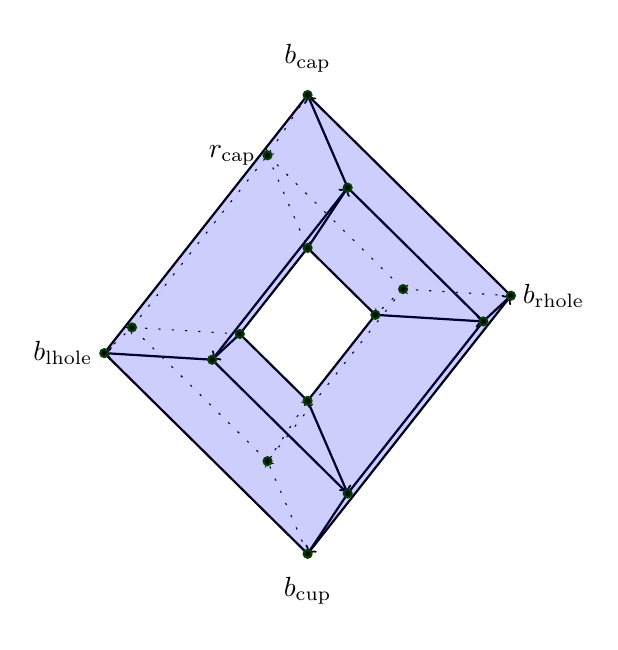
\begin{tikzpicture}%
  [x={(-0.860769cm, -0.121512cm)},
  y={(0.508996cm, -0.205391cm)},
  z={(-0.000053cm, 0.971107cm)},
  scale=1,
  back/.style={loosely dotted, thin},
  edge/.style={->,black, thick},
  line/.style={black, thick},
  facet/.style={fill=blue!95!black,fill opacity=0.1},
  vertex/.style={inner sep=1pt,circle,draw=green!25!black,fill=black,thick}]
\coordinate (r_cap) at (0, -1, 5);
\coordinate (g_cap) at (0, 0, 4 );
\coordinate (o_cap) at (0, 1, 5 );
\coordinate (b_cap) at (0, 0, 6 );

\coordinate (r_cup) at (0, -1, 1);
\coordinate (g_cup) at (0, 0, 2 );
\coordinate (o_cup) at (0, 1, 1 );
\coordinate (b_cup) at (0, 0, 0 );

\coordinate (r_ohole) at (-2, -1, 3);
\coordinate (g_ohole) at (-1, 0,  3);
\coordinate (o_ohole) at (-2, 1,  3);
\coordinate (b_ohole) at (-3, 0,  3);

\coordinate (r_rhole) at (2, -1, 3);
\coordinate (g_rhole) at (1, 0,  3);
\coordinate (o_rhole) at (2, 1,  3);
\coordinate (b_rhole) at (3, 0,  3);

\draw[edge,back] (r_cap) -- (g_cap);
\draw[edge]      (g_cap) -- (o_cap);
\draw[edge]      (o_cap) -- (b_cap);
\draw[edge,back] (b_cap) -- (r_cap);

\draw[edge,back] (r_cup) -- (g_cup);
\draw[edge]      (g_cup) -- (o_cup);
\draw[edge]      (o_cup) -- (b_cup);
\draw[edge,back] (b_cup) -- (r_cup);

\draw[edge,back] (r_ohole) -- (g_ohole);
\draw[edge]      (g_ohole) -- (o_ohole);
\draw[edge]      (o_ohole) -- (b_ohole);
\draw[edge,back] (b_ohole) -- (r_ohole);

\draw[edge,back] (r_rhole) -- (g_rhole);
\draw[edge]      (g_rhole) -- (o_rhole);
\draw[edge]      (o_rhole) -- (b_rhole);
\draw[edge,back] (b_rhole) -- (r_rhole);

\draw[line,back] (r_cap) --   (r_ohole);
\draw[line,back] (r_ohole) -- (r_cup);
\draw[line,back] (r_cup) --   (r_rhole);
\draw[line,back] (r_rhole) -- (r_cap);

\draw[line] (g_cap) --   (g_ohole);
\draw[line] (g_ohole) -- (g_cup);
\draw[line] (g_cup) --   (g_rhole);
\draw[line] (g_rhole) -- (g_cap);

\draw[line] (o_cap) --   (o_ohole);
\draw[line] (o_ohole) -- (o_cup);
\draw[line] (o_cup) --   (o_rhole);
\draw[line] (o_rhole) -- (o_cap);

\draw[line] (b_cap) --   (b_ohole);
\draw[line] (b_ohole) -- (b_cup);
\draw[line] (b_cup) --   (b_rhole);
\draw[line] (b_rhole) -- (b_cap);

\fill[facet] (r_cap) -- (r_ohole) -- (g_ohole) -- (g_cap) -- cycle {};
\fill[facet] (r_cap) -- (r_rhole) -- (g_rhole) -- (g_cap) -- cycle {};
\fill[facet] (r_cap) -- (r_ohole) -- (b_ohole) -- (b_cap) -- cycle {};
\fill[facet] (r_cap) -- (r_rhole) -- (b_rhole) -- (b_cap) -- cycle {};

\fill[facet] (o_cap) -- (o_ohole) -- (g_ohole) -- (g_cap) -- cycle {};
\fill[facet] (o_cap) -- (o_rhole) -- (g_rhole) -- (g_cap) -- cycle {};
\fill[facet] (o_cap) -- (o_ohole) -- (b_ohole) -- (b_cap) -- cycle {};
\fill[facet] (o_cap) -- (o_rhole) -- (b_rhole) -- (b_cap) -- cycle {};

\fill[facet] (r_cup) -- (r_ohole) -- (g_ohole) -- (g_cup) -- cycle {};
\fill[facet] (r_cup) -- (r_rhole) -- (g_rhole) -- (g_cup) -- cycle {};
\fill[facet] (r_cup) -- (r_ohole) -- (b_ohole) -- (b_cup) -- cycle {};
\fill[facet] (r_cup) -- (r_rhole) -- (b_rhole) -- (b_cup) -- cycle {};

\fill[facet] (o_cup) -- (o_ohole) -- (g_ohole) -- (g_cup) -- cycle {};
\fill[facet] (o_cup) -- (o_rhole) -- (g_rhole) -- (g_cup) -- cycle {};
\fill[facet] (o_cup) -- (o_ohole) -- (b_ohole) -- (b_cup) -- cycle {};
\fill[facet] (o_cup) -- (o_rhole) -- (b_rhole) -- (b_cup) -- cycle {};

\begin{scope}[nodes=vertex]
\node[label=left:\( r_{\mathrm{cap}} \)] at (r_cap) {};
\node at (g_cap) {};
\node at (o_cap) {};
\node[label=above:\( b_{\mathrm{cap}} \)] at (b_cap) {};
\node at (r_cup) {};
\node at (g_cup) {};
\node at (o_cup) {};
\node[label=below:\( b_{\mathrm{cup}} \)] at (b_cup) {};
\node at (r_ohole) {};
\node at (g_ohole) {};
\node at (o_ohole) {};
\node[label=right:\( b_{\mathrm{rhole}} \)] at (b_ohole) {};
\node at (r_rhole) {};
\node at (g_rhole) {};
\node at (o_rhole) {};
\node[label=left:\( b_{\mathrm{lhole}} \)] at (b_rhole) {};
\end{scope}
\end{tikzpicture}

\caption{Torus embedded in 3-dimensional space. If you see color in your rendering then black lines trace four square-shaped paths, red ones connect the front square to the middle diamonds, and blue ones connect the back path to the middle ones.}
\label{fig:torus}
\end{figure}

\begin{figure}[htbp]
\centering
% https://q.uiver.app/#q=WzAsMzYsWzEsNCwiXFxidWxsZXQiXSxbMSw2LCJcXGJ1bGxldCJdLFsyLDcsIlxcYnVsbGV0Il0sWzIsNSwiXFxidWxsZXQiXSxbMiwzLCJcXGJ1bGxldCJdLFsxLDgsIlxcYnVsbGV0Il0sWzEsMiwiXFxidWxsZXQiXSxbMywyLCJcXGJ1bGxldCJdLFszLDQsIlxcYnVsbGV0Il0sWzMsNiwiXFxidWxsZXQiXSxbMyw4LCJcXGJ1bGxldCJdLFsyLDEsIlxcYnVsbGV0Il0sWzQsMSwiXFxidWxsZXQiXSxbNSwyLCJcXGJ1bGxldCJdLFs0LDMsIlxcYnVsbGV0Il0sWzUsNCwiXFxidWxsZXQiXSxbNCw1LCJcXGJ1bGxldCJdLFs1LDYsIlxcYnVsbGV0Il0sWzQsNywiXFxidWxsZXQiXSxbNSw4LCJcXGJ1bGxldCJdLFsyLDAsIlxcbWF0aHJte2JhY2t9Il0sWzQsMCwiXFxtYXRocm17ZnJvbnR9Il0sWzEsMCwiXFxtYXRocm17b3V0ZXJ9Il0sWzMsMCwiXFxtYXRocm17aG9sZX0iXSxbNSwwLCJcXG1hdGhybXtvdXRlcn0iXSxbMSwxMCwiXFxidWxsZXQiXSxbMiw5LCJcXGJ1bGxldCJdLFszLDEwLCJcXGJ1bGxldCJdLFs0LDksIlxcYnVsbGV0Il0sWzUsMTAsIlxcYnVsbGV0Il0sWzAsMiwiXFxtYXRocm17dG9wXFwgb2ZcXCBkaWFtb25kc30iXSxbMCw2LCJcXG1hdGhybXtib3R0b21cXCBvZlxcIGRpYW1vbmRzfSJdLFsxLDEsIlxcICJdLFs1LDEsIlxcICJdLFszLDEsIlxcICJdLFswLDEwLCJcXG1hdGhybXt0b3BcXCBvZlxcIGRpYW1vbmRzfSJdLFs0LDMsIiIsMix7InN0eWxlIjp7ImhlYWQiOnsibmFtZSI6Im5vbmUifX19XSxbMywyLCIiLDIseyJzdHlsZSI6eyJoZWFkIjp7Im5hbWUiOiJub25lIn19fV0sWzAsMSwiIiwyLHsic3R5bGUiOnsiaGVhZCI6eyJuYW1lIjoibm9uZSJ9fX1dLFs0LDAsIiIsMSx7ImNvbG91ciI6WzIzNiw5MSw2MF0sInN0eWxlIjp7ImhlYWQiOnsibmFtZSI6Im5vbmUifX19XSxbMCwzLCIiLDEseyJjb2xvdXIiOlsyMzYsOTEsNjBdLCJzdHlsZSI6eyJoZWFkIjp7Im5hbWUiOiJub25lIn19fV0sWzMsMSwiIiwxLHsiY29sb3VyIjpbMjM2LDkxLDYwXSwic3R5bGUiOnsiaGVhZCI6eyJuYW1lIjoibm9uZSJ9fX1dLFsxLDIsIiIsMSx7ImNvbG91ciI6WzIzNiw5MSw2MF0sInN0eWxlIjp7ImhlYWQiOnsibmFtZSI6Im5vbmUifX19XSxbMiw1LCIiLDEseyJjb2xvdXIiOlsyMzYsOTEsNjBdLCJzdHlsZSI6eyJoZWFkIjp7Im5hbWUiOiJub25lIn19fV0sWzEsNSwiIiwxLHsic3R5bGUiOnsiaGVhZCI6eyJuYW1lIjoibm9uZSJ9fX1dLFs2LDQsIiIsMSx7ImNvbG91ciI6WzIzNiw5MSw2MF0sInN0eWxlIjp7ImhlYWQiOnsibmFtZSI6Im5vbmUifX19XSxbNiwwLCIiLDEseyJzdHlsZSI6eyJoZWFkIjp7Im5hbWUiOiJub25lIn19fV0sWzcsOCwiIiwwLHsic3R5bGUiOnsiaGVhZCI6eyJuYW1lIjoibm9uZSJ9fX1dLFs4LDksIiIsMCx7InN0eWxlIjp7ImhlYWQiOnsibmFtZSI6Im5vbmUifX19XSxbOSwxMCwiIiwwLHsic3R5bGUiOnsiaGVhZCI6eyJuYW1lIjoibm9uZSJ9fX1dLFs3LDQsIiIsMCx7ImNvbG91ciI6WzIzNiw5MSw2MF0sInN0eWxlIjp7ImhlYWQiOnsibmFtZSI6Im5vbmUifX19XSxbNCw4LCIiLDAseyJjb2xvdXIiOlsyMzYsOTEsNjBdLCJzdHlsZSI6eyJoZWFkIjp7Im5hbWUiOiJub25lIn19fV0sWzgsMywiIiwwLHsiY29sb3VyIjpbMjM2LDkxLDYwXSwic3R5bGUiOnsiaGVhZCI6eyJuYW1lIjoibm9uZSJ9fX1dLFszLDksIiIsMCx7ImNvbG91ciI6WzIzNiw5MSw2MF0sInN0eWxlIjp7ImhlYWQiOnsibmFtZSI6Im5vbmUifX19XSxbOSwyLCIiLDAseyJjb2xvdXIiOlsyMzYsOTEsNjBdLCJzdHlsZSI6eyJoZWFkIjp7Im5hbWUiOiJub25lIn19fV0sWzIsMTAsIiIsMCx7ImNvbG91ciI6WzIzNiw5MSw2MF0sInN0eWxlIjp7ImhlYWQiOnsibmFtZSI6Im5vbmUifX19XSxbMTEsNCwiIiwwLHsic3R5bGUiOnsiaGVhZCI6eyJuYW1lIjoibm9uZSJ9fX1dLFsxMSw2LCIiLDAseyJjb2xvdXIiOlsyMzYsOTEsNjBdLCJzdHlsZSI6eyJoZWFkIjp7Im5hbWUiOiJub25lIn19fV0sWzExLDcsIiIsMCx7ImNvbG91ciI6WzIzNiw5MSw2MF0sInN0eWxlIjp7ImhlYWQiOnsibmFtZSI6Im5vbmUifX19XSxbMTksMTcsIiIsMCx7InN0eWxlIjp7ImhlYWQiOnsibmFtZSI6Im5vbmUifX19XSxbMTgsMTYsIiIsMCx7InN0eWxlIjp7ImhlYWQiOnsibmFtZSI6Im5vbmUifX19XSxbMTYsMTQsIiIsMCx7InN0eWxlIjp7ImhlYWQiOnsibmFtZSI6Im5vbmUifX19XSxbMTcsMTUsIiIsMCx7InN0eWxlIjp7ImhlYWQiOnsibmFtZSI6Im5vbmUifX19XSxbMTUsMTMsIiIsMCx7InN0eWxlIjp7ImhlYWQiOnsibmFtZSI6Im5vbmUifX19XSxbMTQsMTIsIiIsMCx7InN0eWxlIjp7ImhlYWQiOnsibmFtZSI6Im5vbmUifX19XSxbMTIsNywiIiwwLHsiY29sb3VyIjpbMSw5NSw2MF0sInN0eWxlIjp7ImhlYWQiOnsibmFtZSI6Im5vbmUifX19XSxbMTIsMTMsIiIsMCx7ImNvbG91ciI6WzEsOTUsNjBdLCJzdHlsZSI6eyJoZWFkIjp7Im5hbWUiOiJub25lIn19fV0sWzEzLDE0LCIiLDAseyJjb2xvdXIiOlsxLDk1LDYwXSwic3R5bGUiOnsiaGVhZCI6eyJuYW1lIjoibm9uZSJ9fX1dLFsxNCw4LCIiLDAseyJjb2xvdXIiOlsxLDk1LDYwXSwic3R5bGUiOnsiaGVhZCI6eyJuYW1lIjoibm9uZSJ9fX1dLFsxNCwxNSwiIiwwLHsiY29sb3VyIjpbMSw5NSw2MF0sInN0eWxlIjp7ImhlYWQiOnsibmFtZSI6Im5vbmUifX19XSxbMTUsMTYsIiIsMCx7ImNvbG91ciI6WzEsOTUsNjBdLCJzdHlsZSI6eyJoZWFkIjp7Im5hbWUiOiJub25lIn19fV0sWzgsMTYsIiIsMCx7ImNvbG91ciI6WzEsOTUsNjBdLCJzdHlsZSI6eyJoZWFkIjp7Im5hbWUiOiJub25lIn19fV0sWzE2LDksIiIsMCx7ImNvbG91ciI6WzEsOTUsNjBdLCJzdHlsZSI6eyJoZWFkIjp7Im5hbWUiOiJub25lIn19fV0sWzE2LDE3LCIiLDAseyJjb2xvdXIiOlsxLDk1LDYwXSwic3R5bGUiOnsiaGVhZCI6eyJuYW1lIjoibm9uZSJ9fX1dLFsxNywxOCwiIiwwLHsiY29sb3VyIjpbMSw5NSw2MF0sInN0eWxlIjp7ImhlYWQiOnsibmFtZSI6Im5vbmUifX19XSxbOSwxOCwiIiwwLHsiY29sb3VyIjpbMSw5NSw2MF0sInN0eWxlIjp7ImhlYWQiOnsibmFtZSI6Im5vbmUifX19XSxbMTgsMTksIiIsMCx7ImNvbG91ciI6WzEsOTUsNjBdLCJzdHlsZSI6eyJoZWFkIjp7Im5hbWUiOiJub25lIn19fV0sWzE4LDEwLCIiLDAseyJjb2xvdXIiOlsxLDk1LDYwXSwic3R5bGUiOnsiaGVhZCI6eyJuYW1lIjoibm9uZSJ9fX1dLFs3LDE0LCIiLDAseyJjb2xvdXIiOlsxLDk1LDYwXSwic3R5bGUiOnsiaGVhZCI6eyJuYW1lIjoibm9uZSJ9fX1dLFs1LDI2LCIiLDEseyJjb2xvdXIiOlsyMzYsOTEsNjBdLCJzdHlsZSI6eyJoZWFkIjp7Im5hbWUiOiJub25lIn19fV0sWzEwLDI2LCIiLDEseyJjb2xvdXIiOlsyMzYsOTEsNjBdLCJzdHlsZSI6eyJoZWFkIjp7Im5hbWUiOiJub25lIn19fV0sWzIsMjYsIiIsMSx7InN0eWxlIjp7ImhlYWQiOnsibmFtZSI6Im5vbmUifX19XSxbMTgsMjgsIiIsMSx7InN0eWxlIjp7ImhlYWQiOnsibmFtZSI6Im5vbmUifX19XSxbMjYsMjUsIiIsMSx7ImNvbG91ciI6WzIzNiw5MSw2MF0sInN0eWxlIjp7ImhlYWQiOnsibmFtZSI6Im5vbmUifX19XSxbMjYsMjcsIiIsMSx7ImNvbG91ciI6WzIzNiw5MSw2MF0sInN0eWxlIjp7ImhlYWQiOnsibmFtZSI6Im5vbmUifX19XSxbMjgsMjksIiIsMSx7ImNvbG91ciI6WzEsOTUsNjBdLCJzdHlsZSI6eyJoZWFkIjp7Im5hbWUiOiJub25lIn19fV0sWzE5LDI5LCIiLDEseyJzdHlsZSI6eyJoZWFkIjp7Im5hbWUiOiJub25lIn19fV0sWzEwLDI3LCIiLDEseyJzdHlsZSI6eyJoZWFkIjp7Im5hbWUiOiJub25lIn19fV0sWzUsMjUsIiIsMSx7InN0eWxlIjp7ImhlYWQiOnsibmFtZSI6Im5vbmUifX19XSxbMjgsMjcsIiIsMSx7ImNvbG91ciI6WzEsOTUsNjBdLCJzdHlsZSI6eyJoZWFkIjp7Im5hbWUiOiJub25lIn19fV0sWzI4LDE5LCIiLDEseyJjb2xvdXIiOlsxLDk1LDYwXSwic3R5bGUiOnsiaGVhZCI6eyJuYW1lIjoibm9uZSJ9fX1dLFsyOCwxMCwiIiwxLHsiY29sb3VyIjpbMSw5NSw2MF0sInN0eWxlIjp7ImhlYWQiOnsibmFtZSI6Im5vbmUifX19XSxbMzAsNiwiIiwxLHsic3R5bGUiOnsiYm9keSI6eyJuYW1lIjoiZG90dGVkIn19fV0sWzMxLDEsIiIsMSx7InN0eWxlIjp7ImJvZHkiOnsibmFtZSI6ImRvdHRlZCJ9fX1dLFsyMCwxMSwiIiwwLHsic3R5bGUiOnsiYm9keSI6eyJuYW1lIjoiZG90dGVkIn19fV0sWzIxLDEyLCIiLDAseyJzdHlsZSI6eyJib2R5Ijp7Im5hbWUiOiJkb3R0ZWQifX19XSxbMjIsMzIsIiIsMCx7InN0eWxlIjp7ImJvZHkiOnsibmFtZSI6ImRvdHRlZCJ9fX1dLFsyNCwzMywiIiwwLHsic3R5bGUiOnsiYm9keSI6eyJuYW1lIjoiZG90dGVkIn19fV0sWzIzLDM0LCIiLDAseyJzdHlsZSI6eyJib2R5Ijp7Im5hbWUiOiJkb3R0ZWQifX19XSxbMzUsMjUsIiIsMSx7InN0eWxlIjp7ImJvZHkiOnsibmFtZSI6ImRvdHRlZCJ9fX1dXQ==
\begin{tikzcd}
	& {\mathrm{outer}} & {\mathrm{back}} & {\mathrm{hole}} & {\mathrm{front}} & {\mathrm{outer}} \\
	& {\ } & \bullet & {\ } & \bullet & {\ } \\
	{\mathrm{top\ of\ diamonds}} & \bullet && \bullet && \bullet \\
	&& \bullet && \bullet \\
	& \bullet && \bullet && \bullet \\
	&& \bullet && \bullet \\
	{\mathrm{bottom\ of\ diamonds}} & \bullet && \bullet && \bullet \\
	&& \bullet && \bullet \\
	& \bullet && \bullet && \bullet \\
	&& \bullet && \bullet \\
	{\mathrm{top\ of\ diamonds}} & \bullet && \bullet && \bullet
	\arrow[dotted, from=1-2, to=2-2]
	\arrow[dotted, from=1-3, to=2-3]
	\arrow[dotted, from=1-4, to=2-4]
	\arrow[dotted, from=1-5, to=2-5]
	\arrow[dotted, from=1-6, to=2-6]
	\arrow[draw={rgb,255:red,60;green,73;blue,246}, no head, from=2-3, to=3-2]
	\arrow[draw={rgb,255:red,60;green,73;blue,246}, no head, from=2-3, to=3-4]
	\arrow[no head, from=2-3, to=4-3]
	\arrow[draw={rgb,255:red,250;green,59;blue,56}, no head, from=2-5, to=3-4]
	\arrow[draw={rgb,255:red,250;green,59;blue,56}, no head, from=2-5, to=3-6]
	\arrow[dotted, from=3-1, to=3-2]
	\arrow[draw={rgb,255:red,60;green,73;blue,246}, no head, from=3-2, to=4-3]
	\arrow[no head, from=3-2, to=5-2]
	\arrow[draw={rgb,255:red,60;green,73;blue,246}, no head, from=3-4, to=4-3]
	\arrow[draw={rgb,255:red,250;green,59;blue,56}, no head, from=3-4, to=4-5]
	\arrow[no head, from=3-4, to=5-4]
	\arrow[draw={rgb,255:red,250;green,59;blue,56}, no head, from=3-6, to=4-5]
	\arrow[draw={rgb,255:red,60;green,73;blue,246}, no head, from=4-3, to=5-2]
	\arrow[draw={rgb,255:red,60;green,73;blue,246}, no head, from=4-3, to=5-4]
	\arrow[no head, from=4-3, to=6-3]
	\arrow[no head, from=4-5, to=2-5]
	\arrow[draw={rgb,255:red,250;green,59;blue,56}, no head, from=4-5, to=5-4]
	\arrow[draw={rgb,255:red,250;green,59;blue,56}, no head, from=4-5, to=5-6]
	\arrow[draw={rgb,255:red,60;green,73;blue,246}, no head, from=5-2, to=6-3]
	\arrow[no head, from=5-2, to=7-2]
	\arrow[draw={rgb,255:red,60;green,73;blue,246}, no head, from=5-4, to=6-3]
	\arrow[draw={rgb,255:red,250;green,59;blue,56}, no head, from=5-4, to=6-5]
	\arrow[no head, from=5-4, to=7-4]
	\arrow[no head, from=5-6, to=3-6]
	\arrow[draw={rgb,255:red,250;green,59;blue,56}, no head, from=5-6, to=6-5]
	\arrow[draw={rgb,255:red,60;green,73;blue,246}, no head, from=6-3, to=7-2]
	\arrow[draw={rgb,255:red,60;green,73;blue,246}, no head, from=6-3, to=7-4]
	\arrow[no head, from=6-3, to=8-3]
	\arrow[no head, from=6-5, to=4-5]
	\arrow[draw={rgb,255:red,250;green,59;blue,56}, no head, from=6-5, to=7-4]
	\arrow[draw={rgb,255:red,250;green,59;blue,56}, no head, from=6-5, to=7-6]
	\arrow[dotted, from=7-1, to=7-2]
	\arrow[draw={rgb,255:red,60;green,73;blue,246}, no head, from=7-2, to=8-3]
	\arrow[no head, from=7-2, to=9-2]
	\arrow[draw={rgb,255:red,60;green,73;blue,246}, no head, from=7-4, to=8-3]
	\arrow[draw={rgb,255:red,250;green,59;blue,56}, no head, from=7-4, to=8-5]
	\arrow[no head, from=7-4, to=9-4]
	\arrow[no head, from=7-6, to=5-6]
	\arrow[draw={rgb,255:red,250;green,59;blue,56}, no head, from=7-6, to=8-5]
	\arrow[draw={rgb,255:red,60;green,73;blue,246}, no head, from=8-3, to=9-2]
	\arrow[draw={rgb,255:red,60;green,73;blue,246}, no head, from=8-3, to=9-4]
	\arrow[no head, from=8-3, to=10-3]
	\arrow[no head, from=8-5, to=6-5]
	\arrow[draw={rgb,255:red,250;green,59;blue,56}, no head, from=8-5, to=9-4]
	\arrow[draw={rgb,255:red,250;green,59;blue,56}, no head, from=8-5, to=9-6]
	\arrow[no head, from=8-5, to=10-5]
	\arrow[color={rgb,255:red,60;green,73;blue,246}, no head, from=9-2, to=10-3]
	\arrow[no head, from=9-2, to=11-2]
	\arrow[color={rgb,255:red,60;green,73;blue,246}, no head, from=9-4, to=10-3]
	\arrow[no head, from=9-4, to=11-4]
	\arrow[no head, from=9-6, to=7-6]
	\arrow[no head, from=9-6, to=11-6]
	\arrow[color={rgb,255:red,60;green,73;blue,246}, no head, from=10-3, to=11-2]
	\arrow[color={rgb,255:red,60;green,73;blue,246}, no head, from=10-3, to=11-4]
	\arrow[color={rgb,255:red,250;green,59;blue,56}, no head, from=10-5, to=9-4]
	\arrow[color={rgb,255:red,250;green,59;blue,56}, no head, from=10-5, to=9-6]
	\arrow[color={rgb,255:red,250;green,59;blue,56}, no head, from=10-5, to=11-4]
	\arrow[color={rgb,255:red,250;green,59;blue,56}, no head, from=10-5, to=11-6]
	\arrow[dotted, from=11-1, to=11-2]
\end{tikzcd}

\caption{An inspiration for the torus. Identify the sides and then the top, definitionally, to get the actual torus.}
\label{fig:flattorus}
\end{figure}

This somewhat arbitrary and unfamiliar model of a torus has the helpful property that it is a combinatorial manifold that is somewhat minimal while still being representable by a donut shape. But the donut-shaped version suggests a very different connection than the flat model! Starting with the flat model, we can easily see how to define \( T_1 \) by sliding a link rigidly along the page to the link of some adjacent vertex. Then we can see that transport around any loop is the identity and so \( T_2 \) is always the identity (together with the homotopy \( \refl_\id \) from the identity to itself). So if we imagine a way to visit every face like we did for the octahedron, starting and ending at some basepoint \( v \), we expect to see no net rotation at all of \( Tv \). Later we will call this ``total curvature 0.''

The donut-shaped torus suggests a different connection, one determined by the embedding in 3-space that we have represented. But the easiest way to think about that bundle and its connection and curvature is to wait until we have a proof of the Poincaré-Hopf theorem, so that we can instead compute with a vector field.
\end{comment}

\subsection{Existence of connections}

How confident can we be that we can always define a connection on an arbitrary combinatorial manifold? Two things make the octahedron example special: the link is a 4-gon at every vertex, and every edge extends to a symmetry of the entire octahedron, embedded in 3-dimensional space. This imposed a coherence on the interactions of all the choices we made for the connection, which we can worry may not exist for more complex combinatorial data.

We know as a fact outside of HoTT that any combinatorial surface that has been realized as a triangulated surface embedded in 3-dimensional euclidean space can inherit the parallel transport entailed in the embedding. We could then approximate that data to arbitrary precision with enough subdivision of the fibers of \( T \).

What would a proof inside of HoTT look like? We will leave this as an open question.

